\documentclass[10pt,notitlepage]{article}
\usepackage{graphicx} 
\usepackage{verbatim} 
\usepackage[portuguese]{babel}
\usepackage[utf8]{inputenc}
\usepackage[hmargin=2cm,vmargin=3.5cm,bmargin=2cm]{geometry}


\begin{document}

%%%CAPA%%%
\begin{titlepage}
\begin{figure}
\centering

\includegraphics[scale=0.5]{logo.pdf}
\end{figure}



\begin{center}

Escola de Engenharia \\~  Departamento de Informática \\~ \\~ Licenciatura em Engenharia Informática \\~ \\~ \\~  \\~ \\~ \\~ \\~ \\~ \\~ \\~  


{\Huge Projecto Java - FitnessUM }
\\~ \\~ \\~ \\
Programação Orientada aos Objectos
  \vfill

\begin{figure}[h]
\centering

\end{figure}

\begin{figure}[h]
\centering
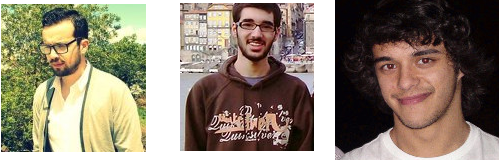
\includegraphics[scale=0.6]{autores.png}
\end{figure}

69303 ~~~~~~~~~~~~~~~~~~ 66822 ~~~~~~~~~~~~~~~~~~~~~ 69854   \\~ Bruno Pereira  ~~~~~~~~ Miguel Guimarães ~~~~~~~João Mano  \\~ \\~ \\~ \\~ \\~ \\~ Braga, Junho de 2014
\end{center}
\end{titlepage}




\tableofcontents

\newpage


\section{Estrutura da aplicação}

\subsection{Actividades}
Foram definidas as seguindes actividades desportivas para a nossa aplicação:

\begin{itemize}
\item Yoga 
\item Aerobics
\item Swimming
\item IndoorCycling
\item Handball
\item Basketball
\item TableTennis
\item Boxing
\item Badminton
\item VolleyBallIndoor
\item Football
\item VolleyBallBeach
\item Running
\item Skating
\item Saling
\item Walking
\item Tennis
\item Skiing
\item Cycling
\item MountainBiking
\item Orienteering
\item Snowboarding
\item Polo
\end{itemize}

\newpage
Para a implementação destas actividades foi usada a seguinte estrutura:



\begin{figure}[ht]
\centering
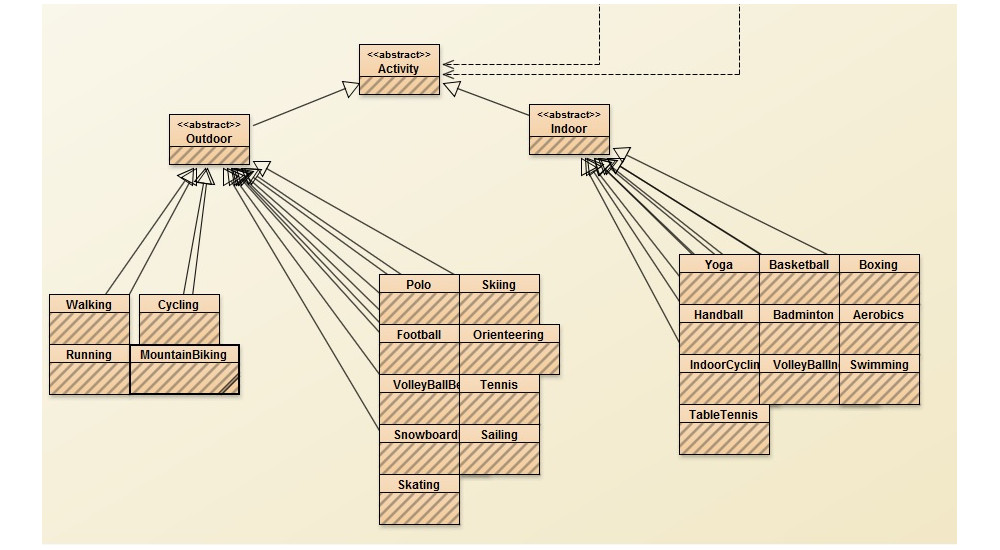
\includegraphics[scale=0.5]{Activity2.jpg}
\caption{Estrutura das actividades}
\label{fig:actividades}
\end{figure}


\subsubsection{Classe abstracta Activity}

Esta é a classe mais abstracta que contem o conceito de actividade. Contém variáveis comuns a todas as actividades:
\begin{itemize}
\item \textit{String name}, nome da actividade criada.
\item \textit{GregorianCalendar date}, data de quando se realizou a actividade.
\item \textit{double timeSpent}, tempo gasto na actividade.
\item \textit{double calories}, campo preenchido pela aplicaçao de uma fórmula.
\end{itemize}
tal como os construtores, \textit{getters} e \textit{setters}.


\subsubsection{Indoor,Outdoor e actividades desportivas}
Todas as actividades desportivas tem um aspecto importante,o clima caso sejam praticadas ao ar livre.\\
Devido a este aspecto foram criadas duas classes abstractas,subclasses de \textit{Activity},para essa distinção.  
\begin{itemize}
\item Outdoor,contém a variável: \textit{String weather}  
\item Indoor
\end{itemize}

Todas as actividades desportivas são subclasses de \textit{Indoor} ou \textit{Outdoor} como exemplicado na figura ~\ref{fig:actividades}.
 
\subsubsection{Comparadores e Iterfaces}
Para organizar as actividades criaram-se dois tipo de comparadores:
\begin{itemize}
\item CompareActivity- Compara a actividade pela data da realização da mesma.
\item CompareActivityByTime- Compara a actividade pelo tempo gasto na realização desta.
\end{itemize}

\begin{figure}[ht]
\centering
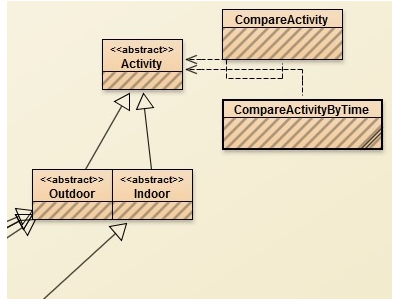
\includegraphics[scale=1]{ComparadorActivity.png}
\caption{Comparador Activity}
\end{figure}

~\\~\\
Como certos desportos usam



\subsection{Utilizadores}
Para destiguir utilizadores regulares de administradores criou-se a seguinte estrutura:
~\\
\begin{figure}[htb]
\centering
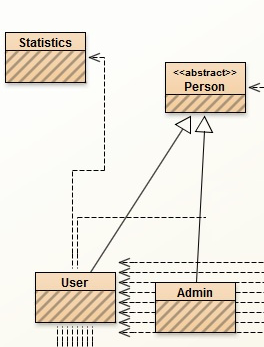
\includegraphics[scale=0.6]{Statsfinal.jpg}
\caption{Estrutura das classes User e Admin}
\end{figure}


\subsubsection{Classe abstracta Person}

~\\~
Classe geral para todo tipo de utilizador. As suas variáveis são:
\begin{itemize}
\item \textit{String email};
\item \textit{String password};
\item \textit{String name};
\item \textit{char gender};
\item \textit{GregorianCalendar dateOfBirth};
\end{itemize}

\subsubsection{Classes User e Admin}

As subclasses de Person referem-se a dois possíveis tipos de utilizador, utilizador normal ou utilizador com privilégios de administrador.\\
A classe Admin não tem métodos ou variáveis adicionais, visto que este tipo de utilizador apenas opera sobre a base de dados da aplicação.\\
A classe User adiciona as seguintes variáveis:
\begin{itemize}
\item \textit{int height};
\item \textit{double weight};
\item \textit{String favoriteActivity};
\item \textit{TreeSet$<$Activity$>$ userActivities} - Actividades realizadas pelo utilizador;
\item \textit{TreeSet$<$String$>$ friendsList} - Lista dos amigos do utilizador;
\item \textit{TreeMap$<$String, ListRecords$>$ records} - Lista dos seus recordes pessoais;
\item \textit{TreeSet$<$String messageFriend} - Lista de pedidos de amizade;
\end{itemize}
Respectivos métodos \textit{getters} e \textit{setters}, construtores e métodos auxiliares para a gestão de amigos/pedidos de amizade, recordes pessoais, das suas actividades e estatísticas relevantes. Ainda contém funções auxiliares para a simulação de eventos.

\subsubsection{Comparators}
O tipo Person tem apenas um comparator:
\begin{itemize}
\item ComparePersonByName - que ordena por ordem alfabética do seu nome.
\end{itemize}
\subsubsection{Statistics}

A classe Statistics é usada para mostrar ao utilizador dados relevantes das suas actividades, estes podem ser descriminados por um dado mês ou por um ano. As suas variáveis são:
\begin{itemize}
\item \textit{double timeSpend};
\item \textit{double calories};
\item \textit{double distance};
\end{itemize}
contém os respectivos métodos \textit{getters} e \textit{setters} e construtores.


\subsection{Recordes Pessoais}
Para registar os recordes chegou-se a estrutura da fig ~\ref{fig:recordes}:
~\\
\begin{figure}[h]
\centering
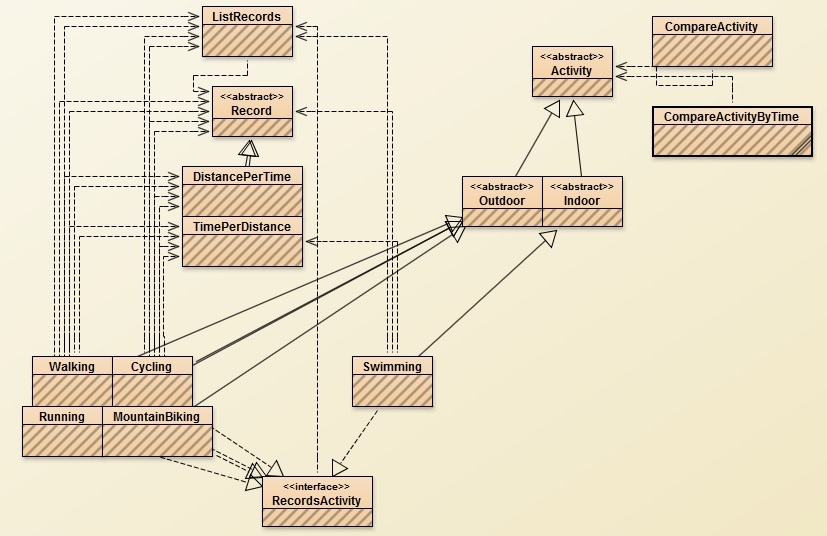
\includegraphics[scale=0.6]{Records.jpg}
\caption{Estrutura dos recordes}
\label{fig:recordes}
\end{figure}


Como se pode verificar na figura ~\ref{fig:recordes}, apenas as seguintes actividades contêm recordes:
\begin{itemize}
\item Running
\item Cycling
\item Walking
\item MountainBiking
\item Swimming
\end{itemize} 


\subsubsection{Classe abstracta Record}

Esta classe representa todos os recordes que o utilizador pode bater.



 Contém apenas uma variável:
\begin{itemize}
\item \textit{String name};
\end{itemize}
métodos construtores, \textit{getName()} e \textit{isEmpty()} que verifica se esse recorde existe ou não.


\subsection{Eventos}

\subsection{Classe abstracta Event}

Classe com o conceito mais abstracto de Evento, contém as variáveis \textit{name}, \textit{tipoActivity}, \textit{location}, \textit{maxParticipants}, \textit{participants}, \textit{deadline}, \textit{date}, \textit{duration}, \textit{participantsList}, \textit{ranking}, \textit{desistentes} e \textit{simula}, respetivos \textit{getters} e \textit{setters} e os vários contrutores. Ainda tem métodos auxiliares para adicionar um \textit{User}, \textit{ranking}, 


\subsection{}


\end{document}

















